\documentclass[journal]{IEEEtran}
\usepackage[utf8]{inputenc}

\usepackage{graphicx}
%\usepackage[caption=false,font=footnotesize]{subfig}
\usepackage{url}
\usepackage{algorithmic}%
\usepackage{algorithm}%
\usepackage{multirow}%
\usepackage{xcolor}%
\usepackage{subcaption}%
\usepackage{placeins}%
\usepackage{circuitikz}%

\usepackage{url}
% Making the references and links clickable
\usepackage{hyperref}
\hypersetup{
    %colorlinks=false,
    pdfborder={0 0 0}
}

\usepackage{xcolor}
\newcommand{\toDo}[1]{\textcolor{red}{#1}}
\newcommand{\mymotor}[2] % #1 = name , #2 = rotation angle
{\draw[thick,rotate=#2] (#1) circle (10pt)
 node[]{$\mathsf M$} 
++(-12pt,3pt)--++(0,-6pt) --++(2.5pt,0) ++(-2.8pt,6pt)-- ++(2.5pt,0pt);
\draw[thick,rotate=#2] (#1) ++(12pt,3pt)--++(0,-6pt) --++(-2.5pt,0) 
++(2.8pt,6pt)-- ++(-2.5pt,0pt);
}

\usepackage{fancyhdr}
\pagestyle{fancy}
\lhead{University of Brasília}
\rhead{\thepage}
\cfoot{Building an H Bridge}
\renewcommand{\headrulewidth}{0.4pt}
\renewcommand{\footrulewidth}{0.4pt}

\begin{document}
    \title{Building an H Bridge}
    
    \author{\IEEEauthorblockN{Bruno H. F. Macedo and
            Gabriel F. P. Araújo}
        \IEEEauthorblockA{
        % \\Laboratório de Automação e Robótica - LARA
        \\Universidade de Brasília - UnB\\
        Brasília - DF - Brasil}
        }
    
    \maketitle
    
    \begin{abstract}
        
        This work presents the design and implementation of an H bridge. The circuit was designed to be used with low power DC motors. This report will present as well the design, prototyping and manufacturing of the board.
                
    \end{abstract}
    
    \begin{IEEEkeywords}
        H bridge, robotics, electric circuits, electronic circuits.        
    \end{IEEEkeywords}
    
 
    \section{\textbf{Introduction}}\label{sec:1}
	DC motors are commonly used in robotics due to it's reduced size, light weight and easy velocity control~\cite{CHAPMAN}, avoiding the use of rectifiers or power inverters. In order to change the orientation of a DC motor, for instance, only the direction of the applied voltage needs to change.

	H bridges (see Figure~\ref{fig:bridge}) are simple electronic circuits used to enable a voltage to be applied across a motor in either direction. Despite it's simplicity H bridges might be used to accomplish more challenging tasks, such as stabilizing distributed energy sources~\cite{H-POWER-QUALITY} and improving power quality in electric vehicles~\cite{H-FILTERING}.

\begin{figure}[h]
\centering
% \begin{subfigure}[b]{0.4\textwidth}
	\centering%
	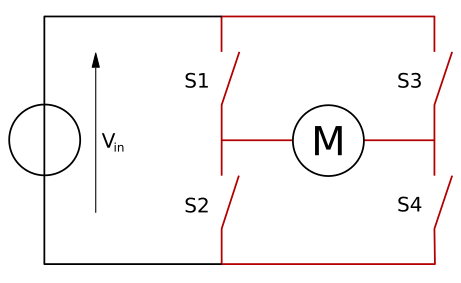
\includegraphics[height=.25\textwidth]{img/H_bridge.png}
	\caption[caption H Bridge]{H Bridge figure borrowed from wikipedia\protect\footnotemark.}
    \label{fig:bridge}%
% \end{subfigure}\hfill
\end{figure}
\footnotetext{\url{https://en.wikipedia.org/wiki/H_bridge}}

    % \input{TORCS_Environment}
    % \input{Related_Works}
    % \input{FSMDriver_ControllerStructure}
    % \input{Genetic_Algorithm}
    % \input{Methodology_Experiments}
    % \input{Analysis_Conclusion}
    % \input{Future_Works}
    
    %\nocite{*}
    \bibliographystyle{IEEEtran}
    \bibliography{Bibliography}
    \toDo{Adequar as referências ao padrão do IEEE: \url{http://www.ieee.org/documents/ieeecitationref.pdf}. Quando
    há 3 ou mais autores colocar et al.}
    
    
    
\end{document}
